% 第 18 题多面体源图的拓扑重绘：上下底面为矩形，侧棱延长形成 E、F。
% 所有长度比例仅为示意；尺寸标签 a,b,c,d 保留，图中不增添 h。
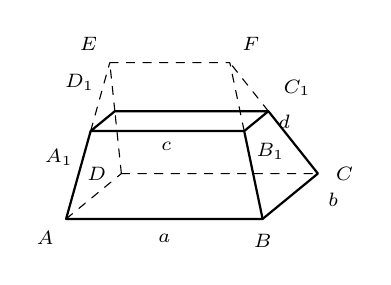
\begin{tikzpicture}[x=.78cm,y=.72cm,line cap=round,line join=round,
  every node/.style={font=\scriptsize}]
  \coordinate (A)  at (0,0);
  \coordinate (B)  at (3.2,0);
  \coordinate (C)  at (4.1,.8);
  \coordinate (D)  at (.9,.8);
  \coordinate (A1) at (.4,1.55);
  \coordinate (B1) at (2.9,1.55);
  \coordinate (C1) at (3.294,1.9);
  \coordinate (D1) at (.794,1.9);
  \coordinate (E)  at (.711,2.756);
  \coordinate (F)  at (2.666,2.756);

  % 可见棱
  \draw[thick] (A)--(B)--(C)--(C1)--(B1)--(A1)--(D1)--(C1);
  \draw[thick] (A)--(A1) (B)--(B1);
  % 隐藏棱
  \draw[dashed] (A)--(D) (D)--(C) (D)--(D1);
  % 侧棱延长线及交点 E、F；与源图一样用虚线表示。
  \draw[dashed] (A1)--(E) (D1)--(E) (B1)--(F) (C1)--(F) (E)--(F);

  % 源图尺寸标签仅标在线段附近，不画尺寸箭头。
  \node at (1.6,-.34) {$a$};
  \node at (4.35,.33) {$b$};
  \node at (1.63,1.28) {$c$};
  \node at (3.55,1.72) {$d$};

  \node[below left=1pt] at (A) {$A$};
  \node[below=2pt] at (B) {$B$};
  \node[right=3pt] at (C) {$C$};
  \node[left=2pt] at (D) {$D$};
  \node[below left=3pt] at (A1) {$A_1$};
  \node[below right=1pt] at (B1) {$B_1$};
  \node[above right=2pt] at (C1) {$C_1$};
  \node[above left=4pt] at (D1) {$D_1$};
  \node[above left=1pt] at (E) {$E$};
  \node[above right=1pt] at (F) {$F$};
\end{tikzpicture}
